% Chapter Template

\chapter{Diseño e Implementación} % Main chapter title

\label{Chapter3} % Change X to a consecutive number; for referencing this chapter elsewhere, use \ref{ChapterX}

A continuación se describe el \textit{hardware} seleccionado para la extensión del circuito cargador, los criterios tomados en cuenta para su selección, el diseño del circuito y su conexión en \ref{sec:hard}. Luego se describe la arquitectura del sistema en \ref{sec:arq} y entra mas en detalle en \ref{sec:firm}, donde se describe el funcionamiento del \textit{firmware}. 

%----------------------------------------------------------------------------------------
%	SECTION 1
%----------------------------------------------------------------------------------------
\section{Hardware}
\label{sec:hard}

%-----------------------------------
%	SUBSECTION 1
%-----------------------------------
\subsection{El Panel Solar}
\label{subsec:panel} 
En el mercado existen distintas soluciones comerciales que se ajustan a las necesidades de cada aplicación. Ofrecen garantía limitada de entre 10 y 25 años y eficiencia de hasta 20 \% para módulos multicelda.
Es importante que los manufacturadores de módulos aseguren un control de calidad en las celdas fotovoltaicas. Estas están clasificadas según los defectos que puedan tener, identificadas con las letras A a la D. Celdas de grado A son aquellas que no presentan defectos visuales y cumplen con las especificaciones de los datos eléctricos \citep{grado}.

El sistema fotovoltaico propuesto originalmente esta basado en módulos con voltaje de 12V y 0.5A. Como medida de mitigación de riesgos, se planteó emplear componentes disponibles en el mercado local, y luego de tener en cuenta factores como grado de calidad (A), eficiencia, costos, tiempo de entrega, soporte pos-venta y al ser de Industria Argentina, se seleccionó el \textit{módulo fotovoltaico policristalino de alto rendimiento KS10T} \citep{solar} de la figura \ref{fig:ks10t} de SOLARTEC S.A. Se trata de paneles fabricados en base a celdas de silicio policristalino de alta eficiencia de conversión de energía (superior al 14\%).

Cuenta con certificado IRAM (Instituto Argentino de Normalización y Certificación), certificados CE (European Union: IEC61215 \textit{Photovoltaic Solar Testing Specifications} y IEC 61730 {\textit{Photovoltaic (PV) Module Safety Qualification}) y RoHs (\textit{DIRECTIVE 2002/95/EC: Restriction of Hazardous Substances}). Éste último le agrega ventaja frente a líderes del mercado internacional que no cumplen con la restricción de determinadas sustancias peligrosas. Sus características se muestran en la tabla \ref{tab:ks10t}. 
%y figura \ref{fig:mecanicas}\footnote{Fuente: SOLARTEC S.A. Todas las distancias están expresadas en mm.}.

La curva de la figura \ref{fig:curva}, muestra la corriente máxima de cortocircuito y la tensión máxima a circuito abierto del módulo \textit{KS10T}. Nótese que es capaz de entregar la tensión hasta exigir el máximo de corriente. Los valores y la curva están dados para condiciones de insolación de 1 KW/m2, masa atmosférica 1.5 y temperatura de celda de 25 \grados C\citep{solar}.

 \begin{figure}[h!]
	\centering
    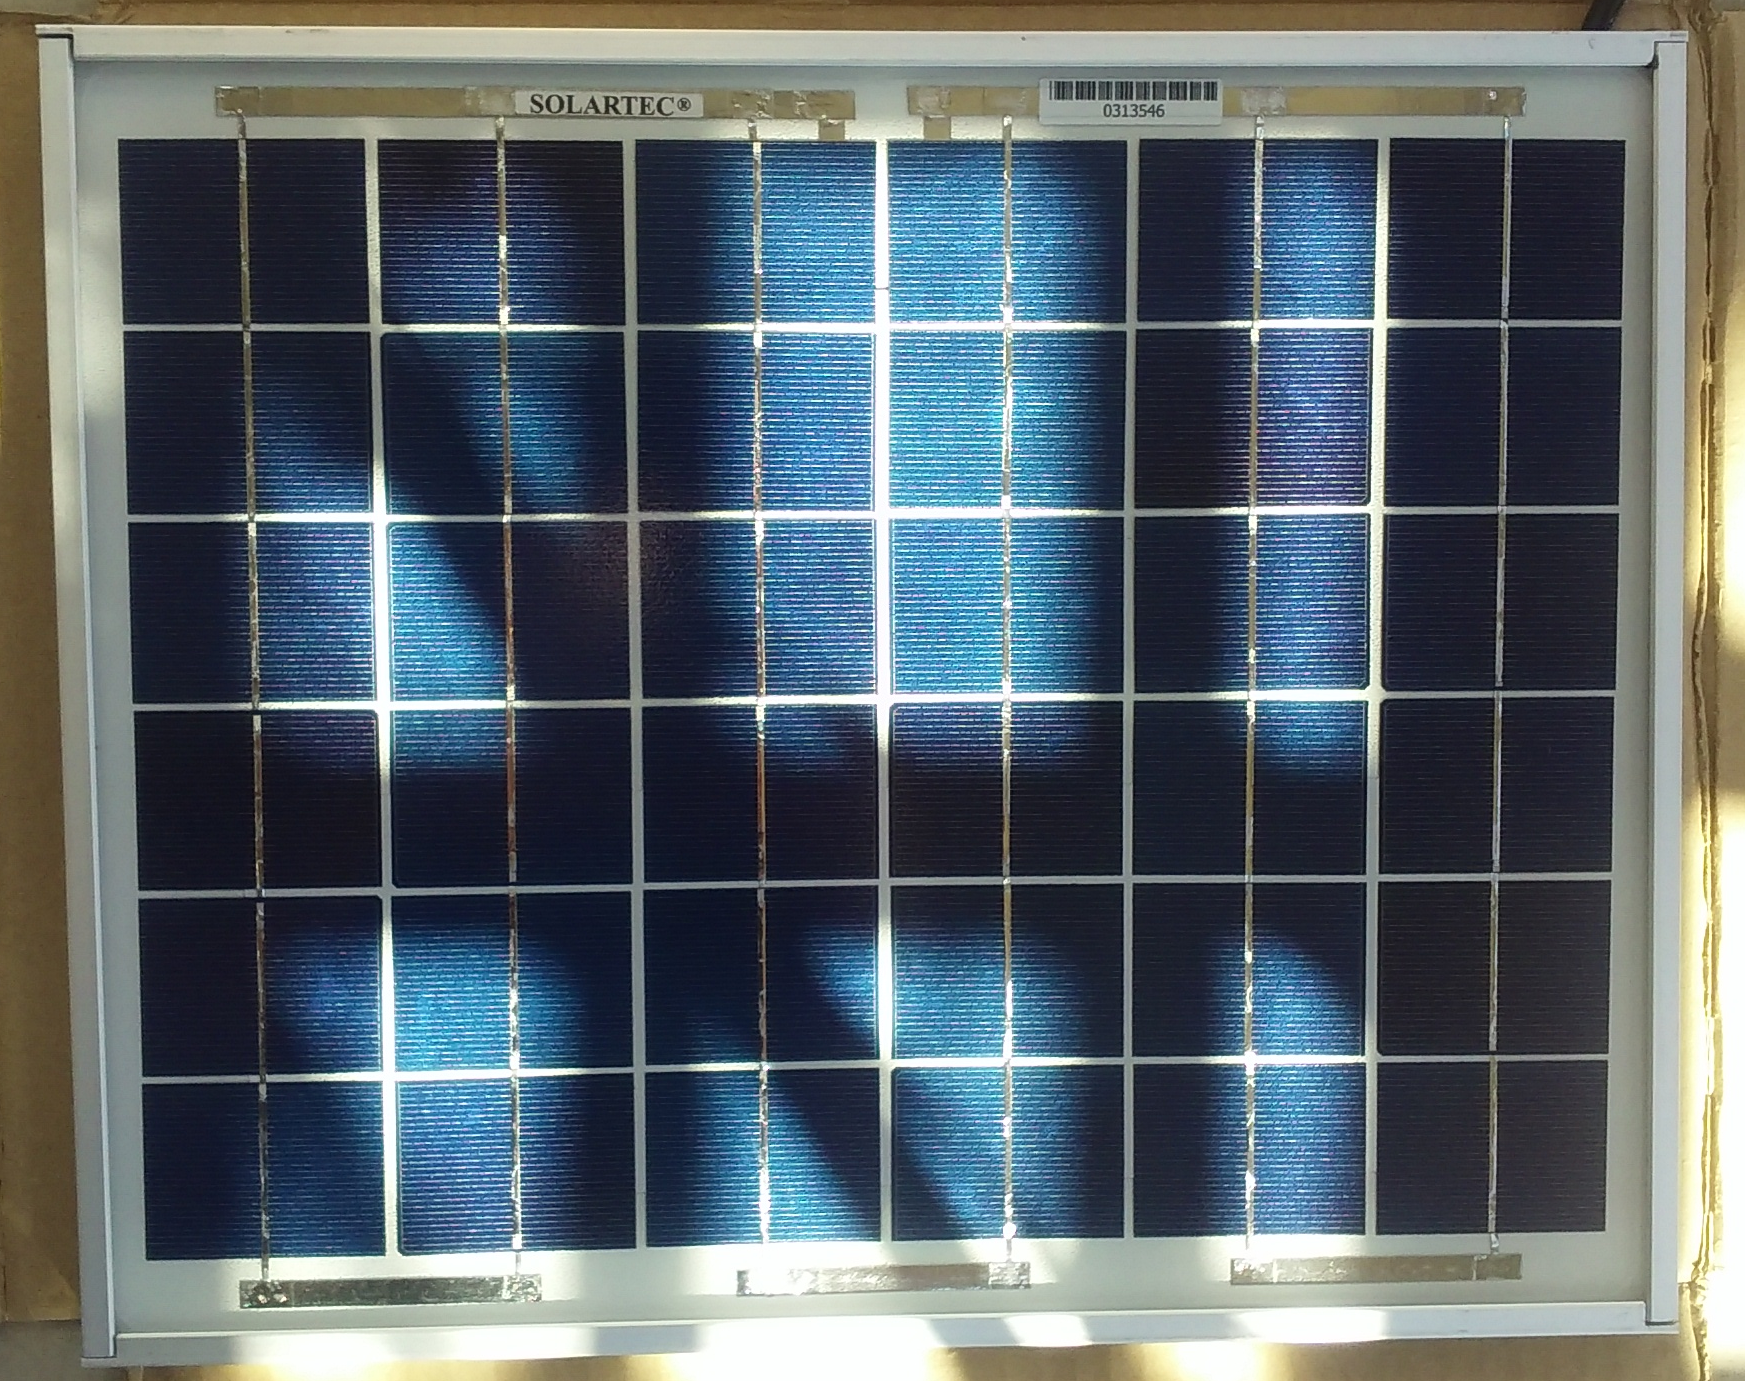
\includegraphics[width=0.6\textwidth]{./Figures/panel.png}
    	\caption{Módulo Fotovoltaico policristalino de alto rendimiento KS10T.}
	\label{fig:ks10t}
\end{figure}

\vspace{10px}

\begin{table}[ht]
	\centering
	\caption{Características del módulo fotovoltaico KS10T}
	\begin{tabular}{@{} l *2c @{}}    \toprule
		\emph{\textbf{Características}} & \emph{\textbf{Valor}} & \emph{\textbf{Unidad}}\\
		\midrule
		Potencia nominal	& 10 	& Wp	\\	
		Tensión a PN		& 17.4	& V\\
		Corriente a PN	& 0.58		& A\\
		Dimensiones		& 301x352x22 	& mm\\
		Peso				& 0.58		& Kg	\\
		\bottomrule
		\hline
	\end{tabular}
	\label{tab:ks10t}
\end{table}


%\begin{figure}[h]
%\centering
%\begin{subfigure}{.5\textwidth}
%%\begin{minipage}{\linewidth}
%  \centering
%    \includegraphics[width=0.5\textwidth]{./Figures/curva.JPG}
%  \caption[a)]{a)\protect\footnotemark}
%	\label{fig:curva}
%%\end{minipage}
%\end{subfigure}%
%\begin{subfigure}{.5\textwidth}
%  \centering
%    \includegraphics[width=0.5\textwidth]{./Figures/mecanicas.JPG}
%  	\caption[b)]{b)\protect\footnotemark}
%	\label{fig:mecanicas}
%\end{subfigure}
%\caption{a)Características eléctricas. b)Características mecánicas.}
%\label{fig:caract}
%\end{figure}

%\begin{figure}[h!]
%	\centering
%    \includegraphics[width=0.5\textwidth]{./Figures/mecanicas.JPG}
%    	\caption{Características mecánicas.}
%	\label{fig:mecanicas}
%\end{figure}

\begin{figure}[h!]
	\centering
    \includegraphics[width=0.6\textwidth]{./Figures/curva.JPG}
    	\caption{Características eléctricas.}
	\label{fig:curva}
\end{figure}

%-----------------------------------
%	SUBSECTION 2
%-----------------------------------
\clearpage
\subsection{Extensión de Circuito Cargador}
\label{subsec:extensión}
Entre las interfaces para el usuario del nodo \textit{Mote LSE} esta el puerto USB, el cual alimenta al circuito de control de carga \textit{bq24080 1-A} con 5V(DC) a través de un conector USB micro-B. Este circuito es el empleado para la carga de la batería de Li-ion de 3.7V y 900mAh.

Es por esto que es necesario emplear una etapa reguladora de voltaje a la salida del panel, para la cual se utiliza el clásico regulador de Fairchild \textit{LM7805} de 1A \citep{7805}. Con unos pocos componentes (un condensador electrolítico como filtro a tierra para señales continuas para moderar la tensión eléctrica y las fluctuaciones de corriente y un condensador de poliéster para filtrar las señales espúreas de alta frecuencia, a la entrada y a la salida) entrega una salida de voltaje entre 4.75V y 5.25V. Además, ofrece protección contra sobrecarga térmica y cortocircuitos y opera entre -40 \grados C y +125 \grados C.

\begin{figure}[h!]
	\centering
    \includegraphics[width=1\textwidth]{./Figures/circuito.jpg}
    	\caption{Diseño de extensión de circuito cargador.}
	\label{fig:circuito}
\end{figure}

Un diseño de circuito alternativo, de montaje superficial, puede hacerse empleando el regulador \textit{TA78M05} de Toshiba Semiconductor. Ver la aplicación del circuito \textit{Current Boost Regulation} en \citep{78M05}.

%Para ver el diseño del PCB de la Extensión de Circuito Cargador, ver \ref{AppendixA}.

%-----------------------------------
%	SUBSECTION 3
%-----------------------------------
\subsection{Diagrama de Conexión}
\label{subsec:conexión}
El siguiente diagrama muestra la conexión entre el panel solar, la extensión del circuito cargador y el nodo \textit{Mote LSE}.

%----------------------------------------------------------------------------------------
%	SECTION 2
%----------------------------------------------------------------------------------------
\section{Arquitectura}
\label{sec:arq}
Cuando se diseña adecuadamente, los drivers de un dispositivo están abstraídos del hardware en sí, para que los usuarios finales, en este caso desarrolladores de software a nivel de aplicación, puedan controlar el hardware cuando una rutina en particular es llamada con el parámetro apropiado (API-CAPI \footnote{Application Programming Interface - Common Application Programming Interface}). Esto se refiere a la interfaz que las aplicaciones pueden usar para comunicarse directamente con el \textit{Mote LSE}.

Primero se usa la función del CMSIS, luego se define en código el handler de la excepción correspondiente, escribiendo en cada entrada del vector la dirección de memoria del handler asociado a la excepción.

A continuación se describe los niveles de abstracción de la arquitectura del firmware, desde los registros primitivos del hardware hasta la aplicación implementada, que incluye varios algoritmos y procedimientos (Ver subsección \ref{subsec:bloques}) que son usados para decidir de forma autónoma el modo de operación, si es necesario cargar la batería y generar alarmas de salud.

El modelo propuesto consiste en una arquitectura de capas (Ver figura \ref{fig:capas}). Los componentes de drivers de dispositivos que dan acceso a los diferentes recursos de hardware del \textit{Mote LSE} y sus funcionalidades están divididos en tres categorías. Los niveles de abstracción se describen en las siguientes capas:

\begin{figure}[h!]
	\centering
    \includegraphics[width=.5\textwidth]{./Figures/arq.png}
    	\caption{Modelo de Capas del Sistema.}
	\label{fig:capas}
\end{figure}


%-----------------------------------
%	SUBSECTION 1
%-----------------------------------
\subsection{HAL}
\label{subsec:hal} 

La capa de abstracción de hardware (en inglés, Hardware Abstraction Layer o HAL) implementa la portabilidad del sistema a otro \textit{hardware} distinto, siendo accesible en un único formato.

\noindent La HAL esta compuesta por:
\begin{itemize}
\item Hardware:
	\begin{itemize}
	\item CMSISv2p00 LPC13xx :Implementa las funciones de acceso al LPC1343.	
	\end{itemize}
\item Board Drivers:
	\begin{itemize}
	\item cc2520.c : Implementa las funciones de acceso al transceiver cc2520.
	\item cc2520.h : Contiene todas las macro que controlan el pin CSn.
	\item ledpul.c : Implementa las funciones de acceso a los leds de la placa.
	\item ledpul.h : Contiene todas las macro que controlan los leds.
	\item bq.c : Implementa las funciones de lectura de estado y control del circuito controlador de carga bq24080.
	\item bq.h : Contiene todas las macro que controla los pines del bq24080.
	\end{itemize}
\end{itemize}
		
%-----------------------------------
%	SUBSECTION 2
%-----------------------------------
\subsection{HIL}
\label{subsec:hil}
La funcionalidad de la HIL no se ve limitada a las plataformas disponibles en la HAL, esto quiere decir que es implementada de una manera que sea independiente del hardware.

\noindent La HAL esta compuesta por:
\begin{itemize}
\item 802.15.4:
	\begin{itemize}
	\item cc2520-mac.c : Implementa las funciones de acceso al medio, arma el FCF e implementa los mecanismos de CSMA/CA.
	\item cc2520-mac.h : Define el tipo de datos necesarios para completar la trama (MHR, MAC Payload, MFR y PHR (Ver figura \ref{fig:data}) asignados en cc2520-task, mientras que el MFR (RSSI y CRC) y el SHR (secuencia de preámbulo y SFD) es implementado por el software embebido del transceiver cc2520 y completa la trama. Especifica el tipo de trama, el modo de direccionamiento MAC (short o extended: 16 o 64 bits) y la estructura de los octetos que forman el PSDU.
	\end{itemize}
\end{itemize}

\vspace{20px}
\begin{figure}[h!]
	\centering
    \includegraphics[width=1\textwidth]{./Figures/data.jpg}
    	\caption{Esquema del formato de la trama de Datos IEEE 802.15.4.}
	\label{fig:data}
\end{figure}

%-----------------------------------
%	SUBSECTION 2
%-----------------------------------
\subsection{APP}
\label{subsec:app}
La capa APP	o de aplicación esta compuesta por:
\begin{itemize}
\item cc2520Task:
	\begin{itemize}
	\item cc2520-task.c : Esta función arma una trama de tipo DATA (formada con los parámetros relativos al 802.15.4 de cc2520-mac.c) y la guarda en el buffer de salida de cc2520. Los parámetros de entrada son la dirección de destino y el payload que contiene todos las mediciones y estados de alarmas. y con la funcion ccTx del cc2520-mac, que se fija en el buffer de tx si contiene un frame y lo transmite. Luego en ccTask implementa una FSM con los estados de enviar, recibir y esperar.
	\item cc2520-task.h : Se incluyeron los estados de operación referentes al transceiver (idle, dataRequest, waitingData, etc)y la función FrameForming para ser utilizada por las capas de aplicación superiores, se define la variable MAXRETRIES que establece el máximo de retransmisiones de una trama y la variables de direccionamiento.
	\end{itemize}
\item monitoreoWsn:	
	\begin{itemize}
	\item monitoreoWsn.c : Implementa las operaciones de medición referentes a cada modo de operación.
	\item monitoreoWsn.h : Define las macros referentes a las mediciones.
	\end{itemize}
\end{itemize}
%----------------------------------------------------------------------------------------
%	SECTION 3
%----------------------------------------------------------------------------------------
\section{Firmware}
\label{sec:firm}
El software embebido, llamado firmware en adelante, fue implementado en lenguaje de programación C y assembler. Éste implementa todas las funciones descriptas en la sección anterior.
 
Como punto de partida, se tomó el \textit{workspace} del Microstack 802.15.4 de la clase práctica de la asignatura Protocolos de Comunicación del Ing. Pablo Ridolfi y se realizaron las modificaciones a nivel de HAL, para soportar el circuito controlador de carga bq24080. Ver \ref{AppendixC}.

\begin{table}[ht]
	\centering
	\caption{Asignación de puertos bq24080 - LPC1343}
	\begin{tabular}{@{} l *3c @{}}    \toprule
		\emph{\textbf{Nombre del puerto bq24080}} & \emph{\textbf{Nombre del puerto LPC1343}} & \emph{\textbf{PIN LPC1343}} & \emph{\textbf{PIN bq24080}}\\
		\midrule
		CE &  PIO3\_ 0 & 36 & 9	\\	
		PG	&  PIO3\_ 1 & 37 & 8\\
		STAT1 &  PIO1\_ 4 & 40 & 3\\
		STAT2 &  PIO2\_ 3 & 38 & 4\\

		\bottomrule
		\hline
	\end{tabular}
	\label{tab:bq}
\end{table}

Se implementaron las funciones para reconocer el estado del circuito según el estado de los pines como figura en la tabla \ref{tab:bq}

\begin{table}[ht]
	\centering
	\caption{Indicador de estado de los pines}
	\begin{tabular}{@{} l *3c @{}}    \toprule
		\emph{\textbf{Estado}} & \emph{\textbf{STAT1}} & \emph{\textbf{STAT2}}\\
		\midrule
		Precarga en progreso &  ON & ON \\	
		Carga rápida en progreso	&  ON & OFF \\
		Carga completa &  OFF & ON \\
		Modo sleep &  OFF & OFF \\

		\bottomrule
		\hline
	\end{tabular}
	\label{tab:bq}
\end{table}

%El \textit{header file} fue incluido en los módulos de la placa (Ver figura \ref{fig:modules}).
%\begin{figure}[h!]
%	\centering
%    \includegraphics[width=1\textwidth]{./Figures/data.jpg}
%    	\caption{Esquema del formato de la trama de Datos IEEE 802.15.4.}
%	\label{fig:modules}
%\end{figure}

Se implementó las funcionalidades de topologías de red WSN en cc2520-task y se agregó otra capa de aplicación que implementa las mediciones y activa las alarmas en el nodo. Todos estos datos son transmitidos al nodo coordinador, para ello emplea la función ccFrameTx, primero guarda los datos de medición en el payload y asigna la dirección del coordinador como dirección destino y guarda la trama formada en el buffer de salida.

Para cumplir con el requerimiento de almacenar en una memoria no volátil los datos de alarma, parámetros monitoreados, tiempo total de uso, y cantidad de ciclos de carga/descarga, éstos son almacenados en la memoria Flash del microcontrolador (la memoria SRAM necesita energía para que perduren los datos). 

A su vez se define un ciclo de trabajo , utlizando un contador junto con el SysTickHandler para iniciar periódicamente la comunicación entre los nodos. 

\noindent La Alarmas que reporta son:
	\begin{itemize}
	\item TempAmbaja : Reporta temperatura de ambiente baja.
	\item TempAmbalta : Reporta temperatura de ambiente alta.
	\item ProyBatrest : En Modo Batería, el nodo calcula la autonomía y utiliza un contador junto con el SysTickHandler con el cual va restando el los pasos del reloj y esta alarma se activa cuando llega a un umbral prefijado.
	\item TensionBat : Se activa cuando la tensión de la batería es menor aun valor prefijado.
	\item NodOffline : Se activa en el nodo master cuando no tiene respuesta de un nodo.
	\end{itemize}

Desde un comienzo se había planificado medir la temperatura de la batería con el bq24080, pero al entrar en detalle de desarrollo con la hoja de datos se encontró que esta funcionalidad no es soportada por la versión utilizada por el hardware, sino la version bq24081, descripto en la misma hoja de datos.

Una opción era emplear un método para medir la temperatura de la batería sin sensores de temperatura, se trata de la medición basada en espectroscopia de impedancia electroquímica\citep{metodo}. Para lo cual se implementaría en el firmware una simple asignación de temperatura basada en la impedancia y el tipo de batería, pero esta medición tampoco es soportada por el bq24080.

Otra opción sería agregarle sensores al Mote LSE, pero modificarlo no es parte del presente trabajo, por las implicaciones de diseño y el tiempo que tomaría su armado y ensamblado. Por lo que se plantea implementar algún otro método en trabajos futuros.

Para ver una descripción del firmware en pseudocódigo y sus principales funciones, ver \ref{AppendixC}.

%Algunas tareas tienen deadlines, otras pueden no tener o pueden tener poca penalidad si no se cumplen.

%#includes

%La función main siempre es llamada cuando el programa se ejecuta por primera vez. De ahi se llama a otras funciones

%-----------------------------------
%	SUBSECTION 1
%-----------------------------------
%\subsection{Diagrama en Bloques}
%\label{subsec:bloques} 
%Diagrama funcional.
%Alarmas.
%Modos.
%Inter PAN
%Módulos. 
%GPIO configurable al recibir un frame de determinadas características (puede esperar tramas de una serie de direcciones - frame filtering)

%-----------------------------------
%	SUBSECTION 1
%-----------------------------------
%\subsection{Descripción de Operaciones}
%\label{subsec:desc} 
%\item en Modo:
%	\begin{itemize}
%	\item cc2520.c : Implementa las funciones de acceso al transceiver cc2520.
%	\item cc2520.h : Contiene todas las macro que controlan el pin CSn.
%	\item ledpul.c : Implementa las funciones de acceso a los leds de la placa.
%	\item ledpul.h : Contiene todas las macro que controlan los leds.
%	\item bq.c : Implementa las funciones de lectura de estado y control del circuito controlador de carga bq24080.
%	\item bq.h : Contiene todas las macro que controla los pines del bq24080.
%	\end{itemize}
%\end{itemize}
%Configuración de cada nodo (Tabla con Parámetros y valores)
%Master: %Configurar como MASTER %Parámetros a ingresar %Diagrama de algoritmo
%Device: %Configurar como DEVICE %Parámetros a ingresar %Diagrama de algoritmo

    
%No se programan tareas con prioridades, es decir que la ejecución de una tarea no sera detenida por el procesador, sin prevaciado y no se implementa tail-chaining ni late-arriving.
%Arquitectura RISK. Modelo Hardvard: Buses separados, pero un unico mapa de memoria que esta predefinido por la arquitectura. Permite agrupar a los perifeicos por funcion y prioridad, lo que simplifica el diseno del microcontrolador y optimiza la velocidad de acceso al mismo.

%Como premisa, modo sleep,
%\textit{wait for interrupt} buena practica
%%(_WFI)



%-----------------------------------
%	SUBSECTION 2
%-----------------------------------
%\subsection{Funcionalidades por Capas}
%\label{subsec:func} 
%\begin{itemize}
%	\item Implementación de funcionalidades en la subcapa PHY
%	
%	\item Implementación de funcionalidades en la subcapa MAC
%
%	\item Implementación de funcionalidades a nivel de aplicación
%	
%\end{itemize}


%-----------------------------------
%	SUBSECTION 4
%-----------------------------------
\subsection{Diagramas de Topologías Implementadas}
\label{subsec:topo} 

Las topologías posibles de implementar son las siguientes:
\begin{figure}[h!]
	\centering
    \includegraphics[width=.8\textwidth]{./Figures/topologia.jpg}
    	\caption{1) Topología estrella. 2)Topología Peer-to-Peer.}
	\label{fig:topo}
\end{figure}

\begin{figure}[h!]
	\centering
    \includegraphics[width=.8\textwidth]{./Figures/cluster.jpg}
    	\caption{Topología árbol de cluster.}
	\label{fig:clust}
\end{figure}

